\documentclass[12pt]{article}

% Pretty much all of the ams maths packages
\usepackage{amsmath,amsthm,amssymb,amsfonts}

% Allows you to manipulate the page a bit
\usepackage[a4paper]{geometry}

\usepackage{authblk}
\usepackage{hyperref}

% Pulls the page out a bit - makes it look better (in my opinion)
\usepackage{a4wide}

% Removes paragraph indentation (not needed most of the time now)
\usepackage{parskip}

% Allows inclusion of graphics easily and configurably
\usepackage{graphicx}

% Provides ways to make nice looking tables
\usepackage{booktabs}

% Allows you to rotate tables and figures
\usepackage{rotating}

% Allows shading of table cells
\usepackage{colortbl}
% Define a simple command to use at the start of a table row to make it have a shaded background
\newcommand{\gray}{\rowcolor[gray]{.9}}

\usepackage{textcomp}

% Provides commands to make subfigures (figures with (a), (b) and (c))
\usepackage{subfigure}

% Provides ways to include syntax-highlighted source code
\usepackage{listings}
\lstset{frame=single, basicstyle=\ttfamily}

% Provides Harvard-style referencing
%\usepackage{natbib}
%\bibpunct{(}{)}{;}{a}{,}{,}

% Provides good access to colours
\usepackage{xcolor}

% Simple command I defined to allow me to mark TODO items in red
\newcommand{\todo}[1] {\textbf{\textcolor{red}{#1}}}

% Allows fancy stuff in the page header
\usepackage{fancyhdr}
\pagestyle{fancy}

% Vastly improves the standard formatting of captions
\usepackage[margin=10pt,font=small,labelfont=bf, labelsep=endash]{caption}

\usepackage{newfloat}
\DeclareFloatingEnvironment[placement={!ht},name=List]{mylist}

\usepackage{tikz}
\usetikzlibrary{calc,3d}
\newcommand{\setxyz}[1]{%
\pgfmathsetmacro{\xone}{cos(180+#1)}%
\pgfmathsetmacro{\yone}{sin(180+#1)}%
\pgfmathsetmacro{\xtwo}{cos(360-#1)}%
\pgfmathsetmacro{\ytwo}{sin(360-#1)}%
}

\usetikzlibrary{decorations.markings}
\tikzstyle arrowstyle=[scale=2]
\tikzstyle directed=[postaction={decorate,decoration={markings,
    mark=at position .82 with {\arrow[arrowstyle]{stealth}}}}]

\pgfmathsetmacro{\xdeg}{30}
\pgfmathsetmacro{\xx}{cos(\xdeg)}
\pgfmathsetmacro{\xy}{sin(\xdeg)}

\pgfmathsetmacro{\ydeg}{150}
\pgfmathsetmacro{\yx}{cos(\ydeg)}
\pgfmathsetmacro{\yy}{sin(\ydeg)}

\pgfmathsetmacro{\zdeg}{90}
\pgfmathsetmacro{\zx}{cos(\zdeg)}
\pgfmathsetmacro{\zy}{sin(\zdeg)}

%
\newcommand*{\email}[1]{%
    \normalsize\href{mailto:#1}{#1}\par
    }


\tikzset{%
mynode/.style={circle,minimum width=.5ex, fill=none,draw}, % no filling
myfillnode/.style={circle,minimum width=.5ex, fill=black,draw}, % fill with black
}

%transforms all coordinates the same way when used (use it within a scope!)
%(rotation is not 45 degress to avoid overlapping edges)
% Input: point of origins x and y coordinate
\newcommand{\myGlobalTransformation}[2]
{
    \pgftransformcm{1}{0}{0.4}{0.5}{\pgfpoint{#1cm}{#2cm}}
}

% draw a 4x4 helper grid in 3D
% Input: point of origins x and y coordinate and additional drawing-parameters
\newcommand{\gridThreeD}[3]
{
    \begin{scope}
        \myGlobalTransformation{#1}{#2};
        \draw [#3,step=2cm] grid (8,8);
    \end{scope}
}

\tikzstyle myBG=[line width=3pt,opacity=1.0]

% draws lines with white background to show which lines are closer to the
% viewer (Hint: draw from bottom up and from back to front)
%Input: start and end point
\newcommand{\drawLinewithBG}[2]
{
    \draw[white,myBG]  (#1) -- (#2);
    \draw[black,very thick] (#1) -- (#2);
}

% draws all horizontal graph lines within grid
\newcommand{\graphLinesHorizontal}
{
    \drawLinewithBG{1,1}{7,1};
    \drawLinewithBG{1,3}{7,3};
    \drawLinewithBG{1,5}{7,5};
    \drawLinewithBG{1,7}{7,7};
}

% draws all vertical graph lines within grid
\newcommand{\graphLinesVertical}
{
    %swaps x and y coordinate (hence vertical lines):
    \pgftransformcm{0}{1}{1}{0}{\pgfpoint{0cm}{0cm}}
    \graphLinesHorizontal;
}

%draws nodes of the grid
%Input: point of origins x and y coordinate
\newcommand{\graphThreeDnodes}[2]
{
    \begin{scope}
        \myGlobalTransformation{#1}{#2};
        \foreach \x in {1,3,5,7} {
            \foreach \y in {1,3,5,7} {
                \node at (\x,\y) [circle,fill=black] {};
                %this way circle of nodes will not be transformed
            }
        }
    \end{scope}
}

\newcommand{\tdcylxy}[5]{% origin x, origin y, origin z, radius, height
    \path (1,0,0);
    \pgfgetlastxy{\cylxx}{\cylxy}
    \path (0,1,0);
    \pgfgetlastxy{\cylyx}{\cylyy}
    \path (0,0,1);
    \pgfgetlastxy{\cylzx}{\cylzy}
    \pgfmathsetmacro{\cylt}{(\cylzy * \cylyx - \cylzx * \cylyy)/ (\cylzy * \cylxx - \cylzx * \cylxy)}
    \pgfmathsetmacro{\ang}{atan(\cylt)}
    \pgfmathsetmacro{\ct}{1/sqrt(1 + (\cylt)^2)}
    \pgfmathsetmacro{\st}{\cylt * \ct}
    \filldraw[fill=white] (#4*\ct+#1,#4*\st+#2,#3) -- ++(0,0,#5) arc[start angle=\ang,delta angle=180,radius=#4] -- ++(0,0,-#5) arc[start angle=\ang+180,delta angle=180,radius=#4];
    \filldraw[fill=white] (#1,#2,#3) circle[radius=#4];
}


\newcommand{\tdcyl}[5]{% origin x, origin y, origin z, radius, height
    \path (1,0,0);
    \pgfgetlastxy{\cylxx}{\cylxy}
    \path (0,1,0);
    \pgfgetlastxy{\cylyx}{\cylyy}
    \path (0,0,1);
    \pgfgetlastxy{\cylzx}{\cylzy}
    \pgfmathsetmacro{\cylt}{(\cylzy * \cylyx - \cylzx * \cylyy)/ (\cylzy * \cylxx - \cylzx * \cylxy)}
    \pgfmathsetmacro{\ang}{atan(\cylt)}
    \pgfmathsetmacro{\ct}{1/sqrt(1 + (\cylt)^2)}
    \pgfmathsetmacro{\st}{\cylt * \ct}
    \filldraw[fill=white] (#4*\ct+#1,#4*\st+#2,#3) -- ++(0,0,#5)
    arc[start angle=\ang,delta angle=-180,radius=#4] -- ++(0,0,-#5)
    arc[start angle=\ang+180,delta angle=180,radius=#4];
    %\draw[dashed] (#4*\ct+#1,#4*\st+#2,#3) -- ++(0,0,#5)
    %arc[start angle=\ang,delta angle=-180,radius=#4] -- ++(0,0,-#5)
    %arc[start angle=\ang+180,delta angle=180,radius=#4]
    %arc[start angle=180+90-\ang,delta angle=180,radius=#4];
    \draw[dashed] (#4*\ct+#1,#4*\st+#2,#3) 
    arc[start angle=180+90-\ang,delta angle=180,radius=#4];
    \filldraw[fill=white] (#1,#2,#3+#5) circle[radius=#4];
}

\newcommand{\tdcylwithbase}[5]{% origin x, origin y, origin z, radius, height
    \path (1,0,0);
    \pgfgetlastxy{\cylxx}{\cylxy}
    \path (0,1,0);
    \pgfgetlastxy{\cylyx}{\cylyy}
    \path (0,0,1);
    \pgfgetlastxy{\cylzx}{\cylzy}
    \pgfmathsetmacro{\cylt}{(\cylzy * \cylyx - \cylzx * \cylyy)/ (\cylzy * \cylxx - \cylzx * \cylxy)}
    \pgfmathsetmacro{\ang}{atan(\cylt)}
    \pgfmathsetmacro{\ct}{1/sqrt(1 + (\cylt)^2)}
    \pgfmathsetmacro{\st}{\cylt * \ct}
    \filldraw[fill=white] (#4*\ct+#1,#4*\st+#2,#3) -- ++(0,0,#5)
    arc[start angle=\ang,delta angle=-180,radius=#4] -- ++(0,0,-#5)
    arc[start angle=\ang+180,delta angle=180,radius=#4];
    %\draw[dashed] (#4*\ct+#1,#4*\st+#2,#3) -- ++(0,0,#5)
    %arc[start angle=\ang,delta angle=-180,radius=#4] -- ++(0,0,-#5)
    %arc[start angle=\ang+180,delta angle=180,radius=#4]
    %arc[start angle=180+90-\ang,delta angle=180,radius=#4];
    \draw[fill=brown,draw=blue,opacity=.8,very thick,line join=round] (#4*\ct+#1,#4*\st+#2,#3) 
    arc[start angle=90-\ang+180,delta angle=180,radius=#4]
    arc[start angle=90-\ang,delta angle=180,radius=#4];
    \filldraw[fill=white] (#1,#2,#3+#5) circle[radius=#4];
}

\newcommand{\tdcylwithlateral}[5]{% origin x, origin y, origin z, radius, height
    \path (1,0,0);
    \pgfgetlastxy{\cylxx}{\cylxy}
    \path (0,1,0);
    \pgfgetlastxy{\cylyx}{\cylyy}
    \path (0,0,1);
    \pgfgetlastxy{\cylzx}{\cylzy}
    \pgfmathsetmacro{\cylt}{(\cylzy * \cylyx - \cylzx * \cylyy)/ (\cylzy * \cylxx - \cylzx * \cylxy)}
    \pgfmathsetmacro{\ang}{atan(\cylt)}
    \pgfmathsetmacro{\ct}{1/sqrt(1 + (\cylt)^2)}
    \pgfmathsetmacro{\st}{\cylt * \ct}
    \filldraw[fill=white] (#4*\ct+#1,#4*\st+#2,#3) -- ++(0,0,#5)
    arc[start angle=\ang,delta angle=-180,radius=#4] -- ++(0,0,-#5)
    arc[start angle=\ang+180,delta angle=180,radius=#4];
    \draw[fill=brown,draw=blue,opacity=.8,very thick,line join=round] (#4*\ct+#1,#4*\st+#2,#3)
    -- ++(0,0,#5)
    arc[start angle=\ang,delta angle=-180,radius=#4] -- ++(0,0,-#5)
    arc[start angle=\ang+180,delta angle=180,radius=#4];
    %arc[start angle=180+90-\ang,delta angle=180,radius=#4];
    \draw[draw=blue,dashed] (#4*\ct+#1,#4*\st+#2,#3) 
    arc[start angle=180+90-\ang,delta angle=180,radius=#4];

    %\draw[fill=brown,draw=blue,opacity=.8,very thick,line join=round] (#4*\ct+#1,#4*\st+#2,#3) 
    %arc[start angle=90-\ang+180,delta angle=180,radius=#4]
    %arc[start angle=90-\ang,delta angle=180,radius=#4];
    \filldraw[fill=white] (#1,#2,#3+#5) circle[radius=#4];
}


\newcommand{\curl}{\operatorname{curl}}
\renewcommand{\div}{\operatorname{div}}
\newcommand{\trace}{\operatorname{tr}}
\newcommand{\diag}{\operatorname{diag}}


\def\b1{{\mathbf 1}}
\def\bv{{\mathbf v}}
\def\bu{{\mathbf u}}
\def\bw{{\mathbf w}}
\def\bb{{\mathbf b}}
\def\bc{{\mathbf c}}
\def\bg{{\mathbf g}}
\def\bh{{\mathbf h}}
\def\br{{\mathbf r}}
\def\bs{{\mathbf s}}
\def\bd{{\mathbf d}}
\def\be{{\mathbf e}}
\def\bp{{\mathbf p}}
\def\bq{{\mathbf q}}
\def\bx{{\mathbf x}}
\def\by{{\mathbf y}}
\def\bz{{\mathbf z}}
\def\bn{{\mathbf n}}
\def\bbf{{\mathbf f}}
\def\bB{{\mathbf B}}
\def\bM{{\mathbf M}}
\def\bV{{\mathbf V}}
\def\bU{{\mathbf U}}
\def\bY{{\mathbf Y}}
\def\bF{{\mathbf F}}
\def\bA{{\mathbf A}}
\def\bB{{\mathbf B}}
\def\bC{{\mathbf C}}
\def\bD{{\mathbf D}}
\def\bN{{\mathbf N}}
\def\bT{{\mathbf T}}
\def\bP{{\mathbf P}}
\def\bQ{{\mathbf Q}}
\def\bS{{\mathbf S}}
\def\bR{{\mathbf R}}
 
\def\bepsilon{{\boldsymbol \epsilon}}
\def\balpha{{\boldsymbol \alpha}}
\def\bdelta{{\boldsymbol \delta}}
\def\blambda{{\boldsymbol \lambda}}
\def\bmu{{\boldsymbol \mu}}
 
 
 
%-----------------------------------------------------------------
\renewcommand{\O}{{\mathcal O}}
\newcommand{\Q}{{\mathcal Q}}
\newcommand{\R}{{\mathcal R}}
\newcommand{\A}{{\mathcal A}}
\newcommand{\B}{{\mathcal B}}
\newcommand{\C}{{\mathcal C}}
\newcommand{\D}{{\mathcal D}}
\newcommand{\F}{{\mathcal F}}
\newcommand{\G}{{\mathcal G}}
\newcommand{\I}{{\mathcal I}}
\newcommand{\J}{{\mathcal J}}
\newcommand{\M}{{\mathcal M}}
\newcommand{\N}{{\mathcal N}}
\newcommand{\X}{{\mathcal X}}
\newcommand{\Y}{{\mathcal Y}}
\newcommand{\calY}{{\mathcal Y}}
\newcommand{\calS}{{\mathcal S}}
\renewcommand{\L}{{\mathcal L}}
\renewcommand{\P}{{\mathcal P}}
 
\newcommand{\V}{\text{\bf V}}
\newcommand{\K}{{\mathcal K}}
\newcommand{\T}{{\mathcal T}}
\newcommand{\E}{{\mathcal E}}

\newcommand{\hatcalK}{\widehat{\mathcal K}}
\newcommand{\hatcalS}{\widehat{\mathcal S}}
\newcommand{\hatA}{\widehat{A}}
%% \newcommand{\grad}{\nabla}
%% \renewcommand{\div}{\text{div}}
%% \renewcommand{\curl}{\text{curl}}
%
%
\def\XVec#1{{\mathbf #1}}
\def\XNorm#1{\left\| #1 \right\|}                       % norm
\def\XIProd#1#2{\left\langle #1 ,~ #2 \right\rangle}    % inner product
 
\def\XM{\mu}
 
\def\XQ{Q}                     % interpolant
\def\Xq#1{\XVec{q}_{#1}}       % rows of Q (interpolation to point #1)
\def\Xu{\XVec{u}}              % unknown vector
\def\Xf{\XVec{f}}              % right-hand-side vector
\def\Xe{\XVec{e}}
\def\Xr{\XVec{r}}
\def\Xx{\XVec{x}}
\def\Xv{\XVec{v}}
\def\Xw{\XVec{w}}
\def\Xn{\XVec{n}}              % normal vector
\def\Xes{\Xe_s}
\def\Xec{\Xe_c}
\def\Xus{\Xu_s}
\def\Xuc{\Xu_c}
\def\Xvs{\Xv_s}
\def\Xvc{\Xv_c}
\def\bone{{\boldsymbol 1}}
\def\bphi{{\boldsymbol \varphi}}
\def\bpsi{{\boldsymbol \psi}}
\def\btheta{{\boldsymbol \theta}}
\def\bchi{{\boldsymbol \chi}}
\def\boldeta{{\boldsymbol \eta}}
\def\bolddelta{{\boldsymbol \delta}}
\def\bsigma{{\boldsymbol \sigma}}
\def\btau{{\boldsymbol \tau }}
\def\bxi{{\boldsymbol \xi }}
\def\bdelta{{\boldsymbol \delta}}
 
\def\Nedelec{N\'ed\'elec\ }

\def\bPi{{\boldsymbol \Pi}}
\def\bPhi{{\boldsymbol \Phi}}

% Standard title, author etc.
%\title{Report 1, 2017 \footnote{This work was supported by ..., grant No. }}
\title{Tensor-product mesh construction in 4D}
\author{Kirill Voronin \\
Portland State University \\
kirill.v.voronin@gmail.com}
%\affil{Portland State University}
%\email{kirill.v.voronin@gmail.com}
\date{}
% Put text on the left-hand and right-hand side of the header
\fancyhead{}
\lhead{Report on the parallel tensor-product mesh generator in 4D}
\rhead{K. Voronin}
\chead{}

\begin{document}

\maketitle

\begin{abstract}
In this text a parallel tensor-mesh generator in 4d is presented. The mesh generator is capable of constructing a space-time cylinder for an arbitrary 3d space mesh in parallel.
The parallel mesh generator was implemented in MFEM, available in CFOSLS repository.
\end{abstract}

\section*{Purpose of this text}
In the text below a simple algorithm is proposed to construct in parallel tensor-product simplicial meshes in 4D and analyzed later on. All in all, it is almost a complete paper (yet unpublished since the results are considered to be weak).
The code is available at the link \cite{cfosls_code}. If you have any questions, feel free to contact the author.
If anyone find this text useful or interesting, one can contact the author for further discussion. The author might be wrong in some of his statements, and will be very grateful for pointing out his mistakes.

Project collaborators:
\begin{itemize}
	\item Panayot Vassilevski (PSU, LLNL), \textbf{project supervisor};
	\item Kirill Voronin, PSU, \textbf{author};
	\item Paulina Sepulveda, (former) PSU;
	\item Chak Shing Lee, LLNL;
	\item Martin Neumueller (Linz University).
	%\item Aidan Hamilton (PSU?)
	%\item Dellyan Kalchev (LLNL?)
\end{itemize}

\section*{Introduction}

Finite element method is nowadays a common approach for solving various application problems in physics which is known first of all for its easy-to-implement methodology. Along with the other closely related approaches, e.g., finite volume methods or discontinuous Galerkin methods finite element method has proved its efficiency by handling complicated problems in numerous applications. Application problems usually require detailed meshes with large number of nodes in order to resolve all geometrical or physical features of the considered domain.

Traditionally, these methods are used for discretization in space whereas different approaches, e.g., finite differences or Runge-Kutta methods, are used for time discretization.
However, in many cases separation of time and space can introduce additional difficulties to the problem, e.g., for problems in time-dependent domains or when conditionally stable time discretization methods are used.  

One of the alternative approaches which has gained much attention and developed greatly recently are space-time methods which provide a simultaneous approximation in both time and space. Apparently, one of the main disadvantages of space-time methods is the increased size of the problem to be solved. However, when combined with appropriate upscaling techniques, these methods can be quite efficient and at the same time avoid some of the drawbacks which are typical for traditional discretization methods.

Certainly, for space-time methods appropriate space-time meshes are to be constructed. While a number of mesh generating software exist for two- and three-dimensional cases, almost none are known to the authors which consider four-dimensional case (three-dimensional space + time). Since space-time approaches introduce an additional dimension to the mesh, it is also important to be able to construct the space-time mesh in parallel. First, this will reduce memory requirements since the space-time mesh as a whole might not fit into the memory of a single computational node. Second, it will reduce the total time for mesh generation.

This paper is focusing on the mesh generating algorithm which constructs tensor-product extension $(d+1)$-dimensional space-time meshes for given $d$-dimensional  (triangular or tetrahedral) space meshes in parallel. In section 1 space-time CFOSLS approach is outlined together with basic discretization details. Extended version of the theoretical background behind the considered formulation can be found in \cite{our_cfosls_paper}. The essence of the paper is mesh generating algorithm is presented in section 2. Apart from mesh generating it is visualization which might be important for space-time approaches. This question is addressed to in section 3. Finally, several numerical experiments in which we study the space-time approximation properties as well as the meshing algorithm performance are presented in section 4.

More pictures and practical usage of the presented generator are available in the report on AMR in CFOSLS \cite{amr_cfosls_report}. 


\section{Space-time CFOSLS}
Consider the following problem in a space-time cylinder $\Omega_T = \Omega \times [0, T]$ where $
\Omega$ is a regular (in the most usual sense) domain:
$$
\frac{\partial S}{\partial t} + \operatorname{div}_x \left( \mathcal{L}(S) \right) = q(\mathbf{x}, t), \quad (\mathbf{x},t) \in \Omega_T
$$
which can be either hyperbolic ($\mathcal{L} = \mathbf{b} S$ with velocity $\mathbf{b}(\mathbf{x}, t)$) or parabolic ($\mathcal{L} = - k \nabla S$) depending on the choice of $\mathcal{L}$.

For this initial boundary value problem we also have the initial condition
$$
S(\mathbf{x},0) = S_0(\mathbf{x})
$$
and appropriate boundary conditions. Specifically, for the hyperbolic problem which is considered as an example in the paper, a correct choice can be
$$
\mathbf{b} \cdot \mathbf{n} = 0, \, \, (\mathbf{x},t) \in \partial \Omega \times [0,T],
$$
i.e., no charasteristics are going inside the domain through the lateral boundary of the space-time cylinder,
together with $\operatorname{div}_{x} \mathbf{b} \geq 0$ in order for the problem to be correctly posed.

Then one can introduce 
$$
\bsigma = \left[ \begin{array}{c} \mathcal{L}(S) \\ S \end{array} \right]
$$
and proceed with the equivalent first order formulation:
$$
\left\{
\begin{array}{c}
\operatorname{div}_{x,t} \bsigma = q \\
\bsigma - 
\left[ 
\begin{array}{c} \mathcal{L}(S) \\ S \end{array}
\right] = 0
\end{array}
\right.
$$
Now, the idea of CFOSLS \cite{CFOSLS} is to consider the above problem above as a minimization problem for the following quadratic functional:
$$
J(\bsigma,S) = \| \bsigma - \left[ \begin{array}{c} \mathcal{L}(S) \\ S \end{array} \right] \|^2_{0,K^{-1}} + \| \operatorname{\div}_{x,t} \bsigma - q \|^2_0
$$
in $H(\div) \times V$ under the constraint
$$
(\operatorname{div}_{x,t} \bsigma, w) = (q, w) \, \, \text{for all} \, \, w \in L_2(\Omega_T).
$$
Here $K = K(\mathbf{x})$ is a symmetric and positive definite matrix coefficient, $\| \cdot \|_0$ (or $\| \cdot \|_{0,K^{-1}}$) denotes the (weighted) $L_2$ norm w.r.t to the space-time domain $\Omega_T$ and $V$ is an appropriate functional space for $S$: $L_2$ in hyperbolic case and $H^1$ in parabolic case. It is assumed implicitly that initial and boundary conditions are incorporated into the definition of the considered functional spaces.

In hyperbolic case, after writing down the minimum conditions for $J(\bsigma,S)$ the scalar unknown $S$  can be eliminated by using the following (assuming for simplicity that $K$ is identity):
$$
\left[ 
\begin{array}{c} \mathbf{b} \\ 1 \end{array}
\right]^T
\left[ 
\begin{array}{c} \mathbf{b} \\ 1 \end{array}
\right]
 S = \left[ 
\begin{array}{c} \mathbf{b} \\ 1 \end{array}
\right]^T \bsigma
$$
Then, the variational form of the problem reads as:
$$
\begin{array}{lll}
((I- \frac{1}{\bb^T\bb} \bb\bb^T) \bsigma,\;\btheta)+(\div_{x,t} \bsigma,\;\div_{x,t} \btheta)+(\lambda,\;\div_{x,t} \btheta)&= (f,\;\div_{x,t} \btheta),&\text{for all }\btheta \in H(\div),\\
(\div_{x,t} \bsigma,\;\mu)&= (f,\mu),&\text{for all }\mu \in L_2.
\end{array}
$$
One can notice that the $\div-\div$ term (the second one in the first equation) can be actually eliminated by changing $\lambda$ (the righthand side of the first equation becomes zero then). This is equivalent to excluding the second term in the definition of the CFOSLS functional $J(\bsigma,S)$.

To approximate the obtained problem in $H(\div)$ - $L_2$ one can use $(d+1)$-dimensional Raviart-Thomas finite elements \cite{RT}. On a $(d+1)$-dimensional element $T$ Raviart-Thomas finite elements of order $k$ are defined as
$$
\mathbf{RT}_k(T) = P_k(T)^{d+1} + \mathbf{x}_{xt} \cdot \tilde{P}_k(T)
$$
where $P_k(T)$ and $\tilde{P}_k(T)$ are the set of polynomials of degree $\leq k$ and set of homogeneous polynomials pf degree $k$ on $T$ and $\mathbf{x}_{xt} = (\mathbf{x},t)^T$. 

Then, the global approximation space for $H(\div)$ is defined as 
$$
\mathbf{RT}_k(\Omega_T, \mathcal{T}_{h\tau}) = \left\{ \mathbf{v} \in L_2(\Omega_T)^{d+1} | \, \mathbf{v} |_T \in \mathbf{RT}_k(T) \, \, \text{for all} \, \, T \in \mathcal{T}_{h\tau} \right\}
$$
whereas a compatible approximation of $L_2$ (so that the pair of spaces satisfied \textit{inf-sup} condition) is then given simply as discontinuous polynomials
$$
Q_k (\Omega_T, \mathcal{T}_{h\tau}) = \left\{ q \in L_2(\Omega_T)^{d+1} | \, q |_T \in P_k(T) \, \, \text{for all} \, \, T \in \mathcal{T}_{h\tau} \right\}.
$$
for a given space-time triangulation $\mathcal{T}_{h\tau}$ of the domain $\Omega_T$. Construction of the space-time triangulations is discussed in the next section.

After approximating the $H(\div) - L_2$ formulation using Raviart-Thomas finite elements one can finally arrive at the linear system which takes the following form:
$$
\left[
\begin{array}{cc}
M + BB^T & B^T \\
B & 0 
\end{array} \right]  
\left[
\begin{array}{c}
\bsigma_h \\
\mu_h
\end{array}
\right]
 = \left[
\begin{array}{c}
B^T f\\
f
\end{array} \right].
$$

\section{Mesh construction}
The developed $(d+1)$-dimensional ($d=2,3$) parallel mesh generator is dedicated for constructing meshes of tetrahedrons (or pentatops) for space-time cylinders given arbitrary triangular(or tetrahedral) meshes (called \textit{base meshes} below) in the cylinder base. The input parameters for the algorithm are: base mesh, number of time slabs and time step. Constructed space-time meshes are essentially tensor-product extensions of the base mesh into the higher-dimensional space. %One of the key concepts here is to use local procedures as mu.

\subsection{Serial algorithm}
Here main steps of serial algorithm are discussed. Although mesh storage formats used by mesh generating software can slightly vary, our implementation is based on MFEM \cite{mfem} framework and therefore we use MFEM mesh format for unstructured meshes as a model. It includes the following key data structures: 
\begin{enumerate}
\item elements (given by vertex indices)
\item boundary elements (given by vertex indices)
\item vertices (given by their coordinates)
\end{enumerate}
Having these data available for the base mesh, one needs to create similar data structures for the space-time mesh. 

\subsubsection{Generating vertices}
In general, one might consider introducing additional nodes inside the time slabs \cite{Behr} in order to produce a mesh which approximates better certain features of the space-time domain. However, in the implemented algorithm we take the viewpoint that such mesh improvements should be incorporated into the refinement strategies which are outside of the scope of the mesh generation. 
Thereby, since no additional vertices are added inbetween the time sections, generation of the space-time vertices is straight-forward. The  space-time vertices are nothing else but $(d+1)$-dimensional duplicates of base mesh vertices with varying time coordinate.

\subsubsection{Generating elements}
The implemented algorithm for generating $(d+1)$-dimensional mesh elements follows the guidelines from \cite{Behr} and \cite{NeumuellerMeshgen}. Elements are generated in an element-by-element fashion by the following local procedure applied to each of the base mesh elements: \\
\textit{Local procedure to generate elements:}
%\begin{mylist}
\begin{enumerate}
	\item[] In a loop over all time slabs:
	\item For a given time slab form a $(d+1)$-dimensional prism with a given base mesh element in the base,
	\item Decompose the prism into $d$ elements (tetrahedrons or pentatops), see Fig.1.
\end{enumerate}
%\caption*{Local procedure}
%\end{mylist}
Thus, each  prism will be decomposed into $(d+1)$-simplices which are the new space-time elements.

\begin{figure}
\begin{minipage}{0.5\textwidth}
\centering
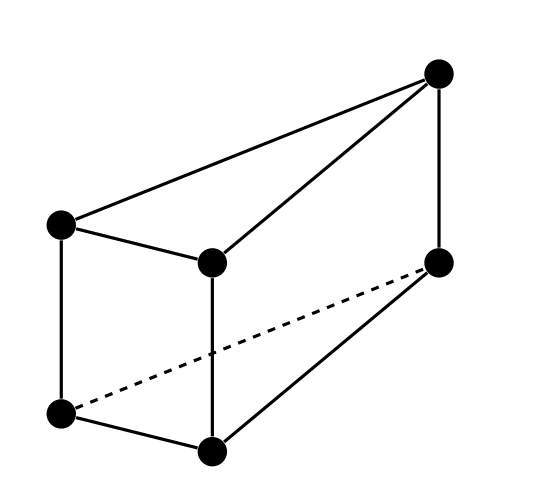
\includegraphics[width = 0.6\textwidth]{prism.png}
\end{minipage}
\hfill
\begin{minipage}{0.5\textwidth}
\centering
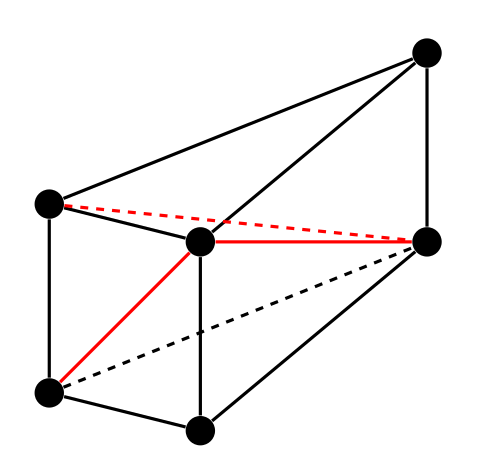
\includegraphics[width = 0.6\textwidth]{triangulated_prism.png}
\end{minipage}
\caption{A space-time prism in three-dimensional case (left) and its tesselation into tetrahedrons (right).}
\end{figure}

For the last step two options were considered and implemented.

\textbf{First approach.} The more general approach \cite{Behr} is to construct a Delaunay triangulation. For creating a Delaunay triangulation one of the standard geometrical packages, e.g., Qhull \cite{qhull} can be used. 
However, one should remember that for a prism with regular faces (in our case the lateral faces are regular) Delaunay tesselation is not unique. This might lead to nonconforming meshes due to the incompatible tesselation of the common faces for neighbouring prisms.
In order to circumvent this, one can joggle (perturb) time coordinates for the vertices in the prism upper base (see Fig.2). In \textit{serial} algorithm the joggling can be random or based on any other information which is global for neighbouring elements, e.g. global vertex indices. For parallel implementation using information which is global for neighbouring elements is not enough since then this idea may lead to additional data transfers and synchronization points. 
Another thing to keep in mind is that due to the round-off errors one might get sliver simplices which should be eliminated afterwards.

\begin{figure}[h]
\centering
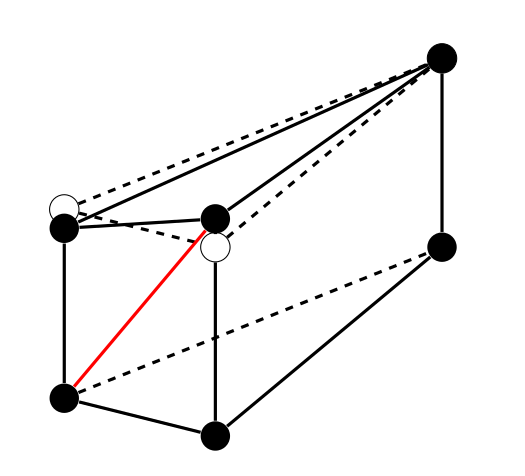
\includegraphics[width = 0.3\textwidth]{perturbed_prism.png}
\caption{A space-time prism with perturbed vertices in three-dimensional case. Now the Delaunay tesselation is unique.}
\end{figure}

Finally, the Delaunay based approach can be written as the following local procedure: \\
\textit{Decomposing $(d+1)$-dimensional prism: Delaunay triangulation}
\begin{enumerate}
	\item Perturb vertex coordinates so that Delaunay triangulation of the prism is unique;
	\item Create a Delaunay triangulation of the prism (using qhull \cite{qhull});
	\item Eliminate sliver (almost degenerate) $(d+1)$-simplices.
	 \end{enumerate}
The elimination can be done by checking the relative simplex volume. The regular volume should be of order $h^3 \tau$ where $h$ is the base mesh step and $\tau$ is the time step.

\textbf{Second approach.} Another approach is to use a standard tesselation \cite{NeumuellerMeshgen} of a $(d+1)$-dimensional prism into $(d+1)$-dimensional simplices. \\
\textit{Decomposing $(d+1)$-dimensional prism: Standard simplex tesselation} 
\begin{enumerate}
	\item If prism vertices in the lower and upper bases are denoted as $A_1, ..., A_k$ and $A_1', ..., A_k'$ correspondingly (see Fig.3), then one can take the following simplices for the prism decomposition:
$\{A_1, ..., A_k, A_1'\}$, $\{A_2, ..., A_k, A_1', A_2'\}$, ..., $\{A_k, A_1', ..., A_k'\}$.
\end{enumerate}

%\begin{figure}[h]
%\centering
%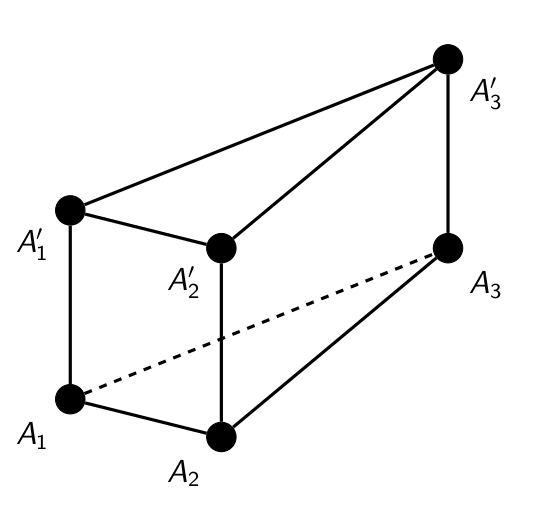
\includegraphics[width = 0.3\textwidth]{ordered_prism.png}
%\caption{A space-time prism with ordered vertices provides a simple way to decompose into tetrahedrons.}
%\end{figure}

\begin{figure}[h]
\begin{minipage}{0.3\textwidth}
\centering
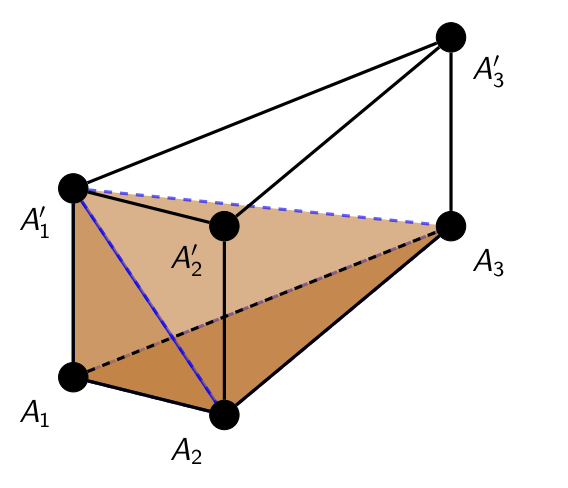
\includegraphics[width = 1.0\textwidth]{first_tetra_prism.png}
\end{minipage}
\hfill
\begin{minipage}{0.3\textwidth}
\centering
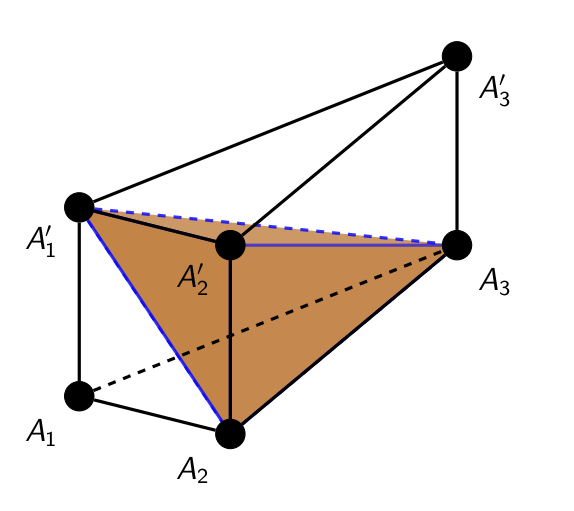
\includegraphics[width = 1.0\textwidth]{second_tetra_prism.png}
\end{minipage}
\begin{minipage}{0.3\textwidth}
\centering
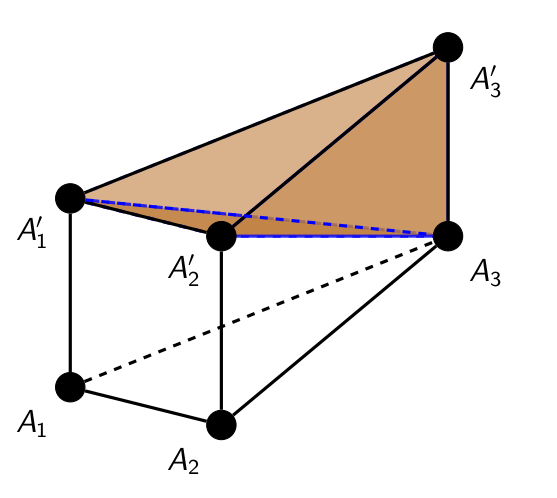
\includegraphics[width = 1.0\textwidth]{third_tetra_prism.png}
\end{minipage}
\caption{Decomposition of a three-dimensional space-time prism into three tetrahedrons based on the vertex numbering.}
\end{figure}


In order to have compatible tesselations across neighbouring elements, the authors of \cite{NeumuellerMeshgen}  suggest to reorder the prism vertices so that the global ordering of vertex indices is preserved. This idea will be slightly modified for the parallel setup.

\subsubsection{Generating boundary elements}

%\begin{figure}
%\hfill
%\begin{minipage}{0.6\textwidth}
%\begin{tikzpicture}%
%    \begin{scope}
%	    \def\height{2.5}
%        \myGlobalTransformation{0}{0};
%        \pgftransformreset
%        \node (A0) at (3,1) [circle,fill=black] {};
%        \node (B0) at (5,0.5) [circle,fill=black] {};
%        \node (C0) at (8,3) [circle,fill=black] {};
%
%        %lower base
%        \draw[black,very thick] (A0) -- (B0);
%        \draw[black,very thick] (B0) -- (C0);
%        \draw[black,dashed,very thick] (A0) -- (C0);
%        \node (A11) at (3,1 + \height - 0.1 * \height) [circle,fill=black] {};
%        \node (B11) at (5,0.5 + \height + 0.15 * \height) [circle,fill=black] {};
%        \node (C11) at (8,3 + \height) [circle,fill=black] {};
%
%		%unperturbed nodes
%        \node (A1) at (3,1 + \height) [mynode] {};
%        \node (B1) at (5,0.5 + \height) [mynode] {};
%        \node (C1) at (8,3 + \height) [mynode] {};
%
%        % old upper base
%        \draw[black,dashed,very thick] (A1) -- (B1);
%        \draw[black,dashed,very thick] (B1) -- (C1);
%        \draw[black,dashed,very thick] (A1) -- (C1);
%
%        % upper base
%        \draw[black,very thick] (A11) -- (B11);
%        \draw[black,very thick] (B11) -- (C11);
%        \draw[black,very thick] (A11) -- (C11);
%
%        %lateral edges
%        \draw[black,very thick] (A0) -- (A11);
%        \draw[black,very thick] (B0) -- (B1);
%        \draw[black,very thick] (B1) -- (B11);
%        \draw[black,very thick] (C0) -- (C11);
%        %\draw[black,dashed] (B11) -- (B1);
%        
%        %diagonals example
%        %\draw[red,very thick] (B0) -- (C11);
%        %\draw[red,very thick] (A11) -- (B0);
%        \draw[red,very thick] (A0) -- (B11);        
%        
%        
%        
%	    %\graphThreeDnodes{0}{0};
%	\end{scope}
%\end{tikzpicture}
%\caption{Prism tesselation in 3D.}
%\end{minipage}
%\hfill
%\end{figure}


It is easy to notice that the boundary of the space-time mesh consists of the following parts: 
\begin{enumerate}
	\item lower cylinder base, 
	\item upper cylinder base,
	\item element faces whose projections onto the base mesh along the time direction are boundary elements of the base mesh.
\end{enumerate}
The first and second types of boundary elements can be added to the structure for space-time boundary elements at any moment. The key question is then how to handle the third type, i.e., how to determine whether any faces of a given base mesh element belong to the boundary of the base mesh. Again, here several options are possible. 

In case when no face-to-boundary connection table (or any equivalent) is available for the base mesh, one can create a list of all base mesh boundary elements and look up in it for each base face which leads to $O(\,n_{f} \cdot \log \, n_{be})$ operations where $n_{f}$ is the number of faces and $n_{be}$ is the number of boundary elements in the base mesh.

Usually, however, face-to-boundary connection table is known so one can simply use it for checking if the given base element's face belongs to the boundary.

\subsection{Parallel algorithm}
As an input for the parallel algorithm we consider a base mesh which is already distributed among the processes. In this case the distributed mesh parts (for our model data structures in MFEM) have their own local-to-process numbering as well as data structures for shared entities: faces, planars (in 4D), edges, and vertices.

The parallel implementation consists of two main steps which are:
\begin{enumerate}
	\item generating local parts of the space-time mesh on the processes, 
	\item setting up communication structures governing the shared entities between processes.
\end{enumerate}
Certainly, local parts are generated via the serial algorithm on each process.

As for the shared entities, one should notice that as soon as shared entities are known for the base mesh, the shared entities can be also defined for the space-time elements by considering projections of space-time entities onto the base. For example, shared planars in 4D (which are essentially triangles) can be defined as those planars whose projection on the base is either a shared edge or a shared face (triangle) of the tetrahedral base mesh. 

It is quite easy to compute the total number of shared planars for each process. Consider a lateral face of the 4D space-time prism (which itself is a three-dimensional prism in 4D) decomposed into three tetrahedrons, see Fig.4. There are $2$ bases and $2$ inner triangles which are projected onto the same base triangle. In addition, for each lateral face of the considered 3D prism (which is a rectangle in 4D), there are  $2$ triangles which are projected onto the same base edge.

\begin{figure}[h]
\begin{minipage}{0.5\textwidth}
\centering
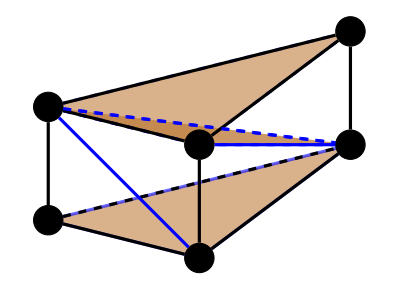
\includegraphics[width = 0.6\textwidth]{planars1_prism.png}
\end{minipage}
\hfill
\begin{minipage}{0.5\textwidth}
\centering
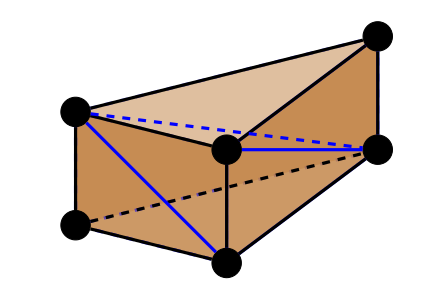
\includegraphics[width = 0.6\textwidth]{planars2_prism.png}
\end{minipage}
\caption{Two types of shared planars in the lateral face which can be considered as a three-dimensional prism. Projections of the planars onto the base plane are eigher base mesh elements (left) or base mesh edges (right).}
\end{figure}


Similarly, knowing shared entities for the base mesh one can define the number of all shared space-time entities via projections:
$$
n_{shared \, faces, d+1} = d \cdot n_{steps} \cdot n_{shared \, faces, d}
$$
$$
n_{shared \, edges, d+1} = (2 \cdot n_{steps} + 1 ) \cdot n_{shared \, edges, d} + n_{steps} \cdot n_{shared \, vertices, d}
$$
$$
n_{shared \, vertices, d+1} = (n_{steps} + 1) \cdot n_{shared \, vertices, d}
$$
$$
n_{shared \, planars, 4} = (2 \cdot n_{steps} + (n_{steps} + 1)) \cdot n_{shared \, faces, 3} + 2 \cdot n_{steps} \cdot n_{shared \, edges, 3}
$$
Here $n_{steps}$ is the number of time slabs in the space-time cylinder, subscripts $d$ and $d+1$ correspond to the space-time and base meshes.

For example, generation of shared planars can be done by performing the following: \\
\textit{Creating shared planars for the space-time mesh:}
\begin{enumerate}
	\item[] In a loop over space-time planars
	\item Project the given planar onto the base. 
	\item Look in the set of shared edges and shared faces of the base mesh for the projection. If found, add a shared planar.
\end{enumerate}

The look-up in the set of base mesh shared entities (step 3 above) implies $O(\,n_{entity, d+1} \cdot \log \, n_{shared entities,d})$ operations. The reason for loops over space-time entities is that if standard routines are used for generating faces, edges and planars, one does not know in advance how they are ordered. As a possible improvement, one could reimplement these generating routines so as to know which space-time entities will be shared.

Special care should be taken so that for each group of the processes which share any mesh entities, the order in which shared entities appear in the lists is the same for all processes in the group (requirement by MFEM).
Another important requirement is to ensure compatible orientation of shared entities across the neighbouring processes and at the same time preserve the local-to-entity indices ordering which can be required by refinement routines. 

In comparison to serial case, parallel setup introduces one additional complication related to the mesh compatibility across neighbouring processes. Usually, mesh parts are handled by different processes and have their own local-to-process vertex numbering. Therefore, one needs to ensure compatibility of the mesh across neighbouring mesh parts which is no longer preserved if one uses local-to-process vertex numbering.

\begin{figure}[h]
\centering
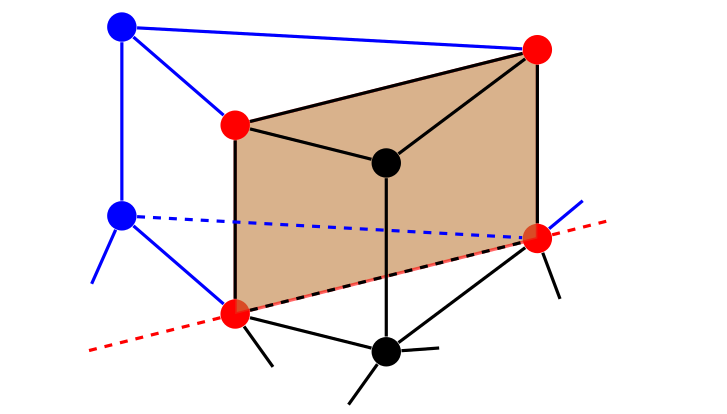
\includegraphics[width = 0.4\textwidth]{shared_face_prism.png}
\caption{A shared face between two neighboring space-time prisms in 3D is essentially a rectangle (with red vertices). The same diagonal should be chosen in the rectangle to ensure mesh compatibility. }
\end{figure}


Here one can notice that in general it is not required to have exactly the same vertex perturbation for common vertices across neighbouring elements and processes in Delaunay triangulation. The same is true for the vertex ordering if one uses simple prism decomposition into simplices. However, in any case one still needs to generate a compatible triangulation.

The simple solution is to use local-to-element ``geometric'' ordering of vertices. That is, one can just reorder the vertices so that the following ``lexicographical'' order is preserved: vertex A is said to be ``larger'' than vertex B if $x$-coordinate of A is larger of $x$-coordinate of B, or their $x$-coordinates are equal and the next coordinate of A is larger than the next one of B, etc. For example, vertex $(0.0; 1.0; 2.0)$ is larger than $(0.0; 1.0; 0.0)$, but less than $(0.0; 2.0; 1.0)$. 

Thus, vertex joggling can be defined to be proportional to the vertex index in this ordering or this ordering can be directly used in simplex decomposition described above. The same trick can be used whenever one needs to orient a space-time entity. Namely, the orientation can be said to be ``positive'' if its vertex ordering is an even permutation of the ``geometric'' ordering defined above.

\textbf{Remark.} The presented algorithm is completely parallel since the local procedures depend only on the local-to-process data. The only communication and synchronization point is required in the very end while finalizing the communication structures which are, for example, communicators for groups of processes which share some entities.

\section{Visualization}
For space-time meshes in 4D it is also important to visualize the obtained results. A common approach  is to slice the space-time domain by a set of hyperplanes defined by $t=t_k$ for a series of time moments $t_k$. The intersection of the $(d+1)$-dimensional space-time mesh and a hyperplane is a $d$-dimensional mesh (called \textit{slice mesh} below). For tetrahedral and pentatop meshes the slice mesh consists of two types of cells: triangles/quadrilaterals in 3D and tetrahedrons/wedges in 4D (see Fig.6).

\begin{figure}[h]
\begin{minipage}{0.5\textwidth}
\centering
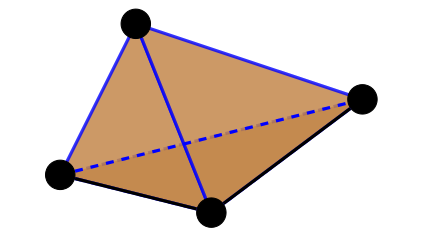
\includegraphics[width = 0.6\textwidth]{tetra.png}
\end{minipage}
\hfill
\begin{minipage}{0.5\textwidth}
\centering
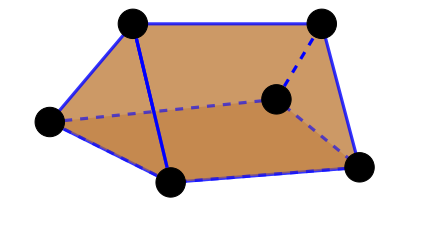
\includegraphics[width = 0.6\textwidth]{wedge.png}
\end{minipage}
\caption{Two types of slice mesh cells in 4D: tetrahedrons (left) and wedges(right).}
\end{figure}


In \cite{NeumuellerViz} an approach based on cutting edges of the mesh elements was presented. The idea is the following: \\
\textit{Local procedure to compute the slice mesh cells:}
\begin{enumerate}
	\item Check whether a considered space-time element is intersected by a given hyperplane.
	\item If it is intersected, two cell types are possible: a tetrahedron or a wedge in 4D, or a triangle or a quadrilateral in 3D. 
	\item The vertices of the slice mesh cell can be computed by intersecting each edge of the space-time element with the hyperplane, see Fig. 7. This can be done by solving a small local system of linear algebraic equations \cite{NeumuellerViz}.
\end{enumerate}

\begin{figure}[h]
\centering
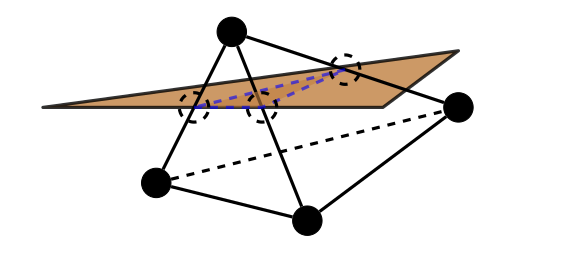
\includegraphics[width = 0.3\textwidth]{sliced_tetra.png}
\caption{An example of slicing a space-time element for a three-dimensional case. The slice cell in 3D is in general either a triangle or a quadrilateral.}
\end{figure}


The procedure can be implemented in parallel while the final output can be processed, e.g., by ParaView \cite{paraview} using unstructured VTK \cite{vtk} or any other standard format. An example of a slice mesh distributed over two parallel processes is presented in Figures 1 and 2. The slice mesh consists of tetrahedrons and wedges. The space-time domain for this mesh was a cylinder with three-dimensional ball in the base:
$$
\Omega_T = \left\{ (x,y,z,t) | \, x^2+y^2+z^2 \leq 1, t \in [0,1]  \right\}.
$$
In Fig.1 local-to-process mesh parts are shown for the slice with $t=0.1$ plane and in Fig. 2 the mesh slices for $t = 0.1$ and $t=0.4$ are shown.

\begin{figure}[!htb]
\minipage{0.48\textwidth}
  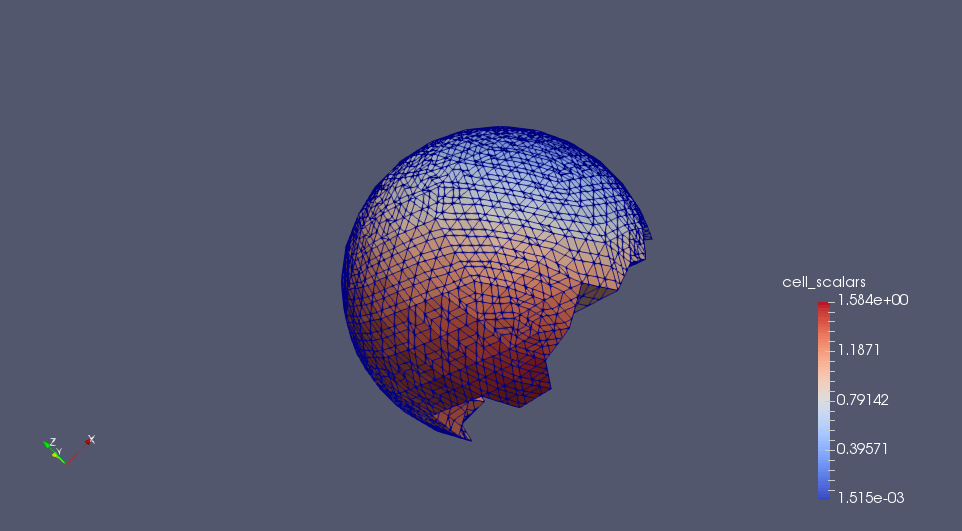
\includegraphics[width=\linewidth]{mesh_1part.png}
%  \caption{A really Awesome Image}\label{fig:awesome_image1}
\endminipage\hfill
\minipage{0.48\textwidth}
  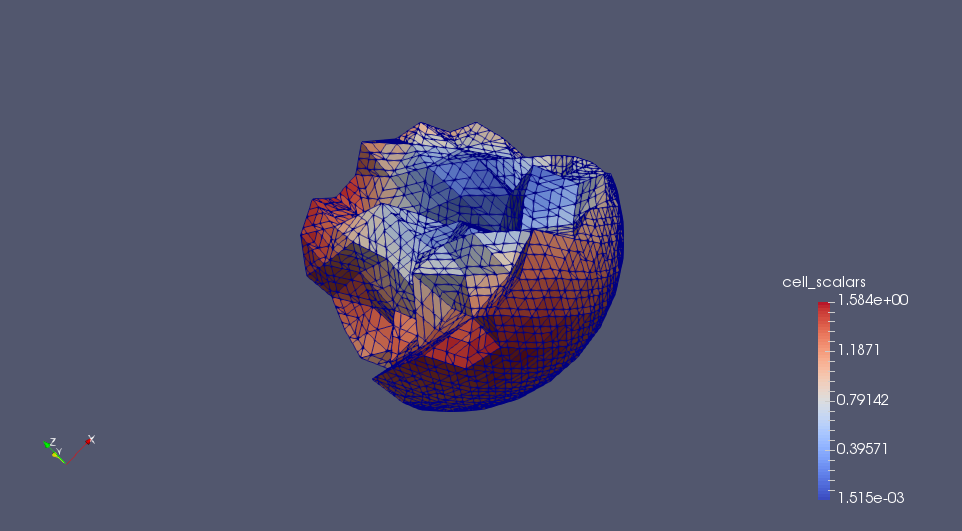
\includegraphics[width=\linewidth]{mesh_2part.png}
%  \caption{A really Awesome Image}\label{fig:awesome_image2}
\endminipage\hfill
\caption{Slice mesh for $t = 0.1$: process 0 (left) and process 1 (right).}
\end{figure}

\begin{figure}[!htb]
\minipage{0.48\textwidth}%
  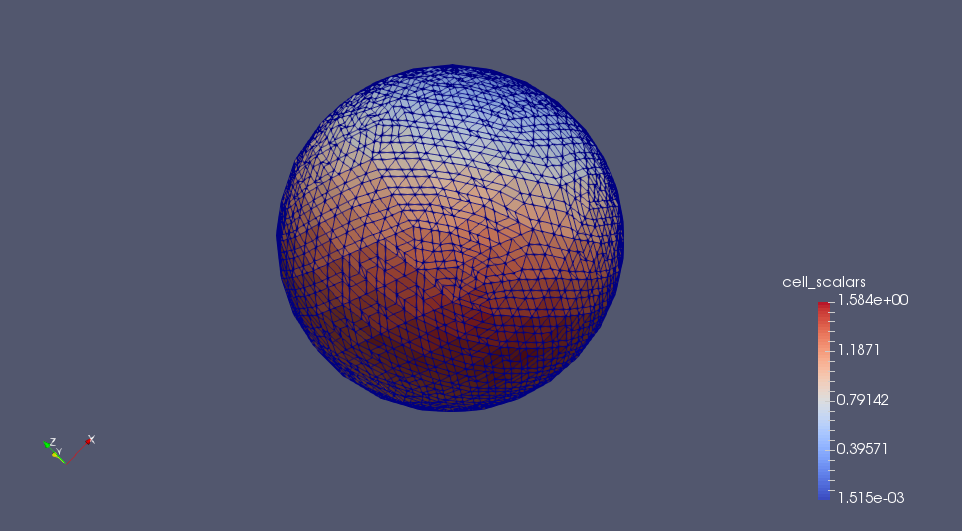
\includegraphics[width=\linewidth]{mesh_bothparts.png}
%  \caption{A really Awesome Image}\label{fig:awesome_image3}
\endminipage\hfill
\minipage{0.48\textwidth}%
  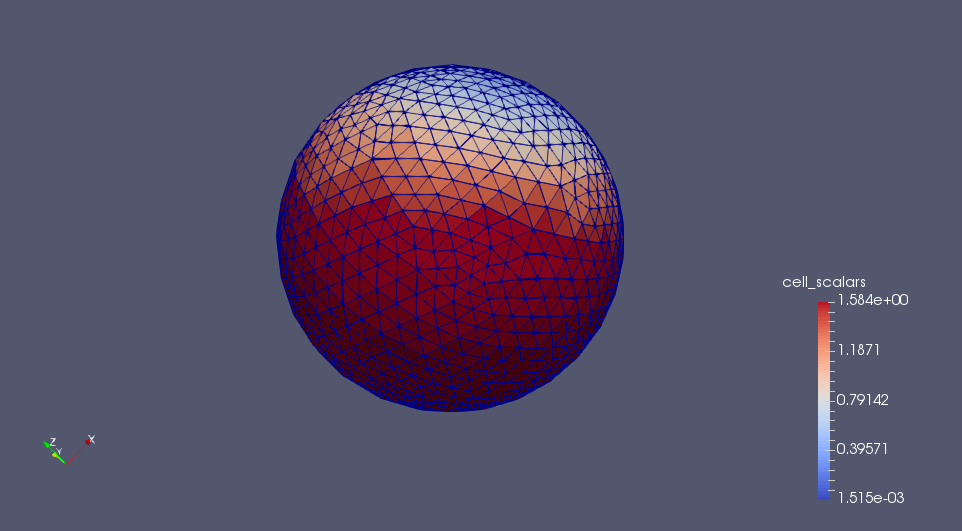
\includegraphics[width=\linewidth]{mesh_bothparts_moment2.png}
%  \caption{A really Awesome Image}\label{fig:awesome_image3}
\endminipage
\caption{Slice mesh for $t=0.1$ (left) and $t = 0.5$ (right).}
\end{figure}


\section{Numerical experiments}

Numerical experiments were perfomed using Coeus cluster \cite{coeus} at Portland Institute of Computational Science (PICS). %The computational nodes used for numerical experiments have the following specification: Intel Xeon ???, GHz, RAM, Infiniband ...

\subsection{Mesh generator}
In general, time for solving the linear system is usually higher than time for mesh generation. Hence the goal of the performance testing for mesh generator is to show that the implemented mesh generating algotihm scales well and hence will not be a performance bottleneck when the number of processes will increase. As already mentioned, the presented algorithm requires very few communication between parallel processes and its nature is essentially parallel since it mainly consists of local procedures. Hence, one should expect it to show a very good scaling with respect to the number of processes. Time and memory scalability of the mesh generator are shown by several simple examples below.

In Table 1  time scalability for space-time mesh generation is presented for a mesh constructed using $n_{proc}$ number of MPI processes from a base mesh with 114,688 elements and 40 time slabs which result in 18,4 mln of elements for the space-time mesh. In the second column  configuration of the parallel system is given as $n \times m$, where $n$ is the number of computational nodes and $m$ is the number of cores per node. In the third column the mesh generation time is presented without considering the construction of the base mesh or doing any additional refinements afterwards. The last column shows the ratio of times between the considered configuration and the previous one (with the ideal ratio being proportional to the change in the number of computational cores which is two in the table).


%Initial 3D mesh: orthotope3D\_fine.mesh with 4 serial refinements \\
%Nelem(3D): 114,688 \\
%Nsteps: 40 \\
%Nelem(4D): 36,700,160 \\ ?? wrong, should be a half of this
%time: for converting 3D to 4D \\
%accel: ratio of times for two consecutive configurations

\begin{center}
\captionof{table}{Parallel mesh generator: Timing} 
\begin{tabular}{|c|c|c|c|}
\hline
$n_{proc}$ & configuration 		& time (s)	& ratio \\
\hline
 1   	   & 1$\times$1 		& 301 		& -		\\
\hline
 2   	   & 2$\times$1 		& 144 		& 2.1	\\
\hline
 4		   & 4$\times$1			& 71  		& 2.02	\\
\hline
 8		   & 8$\times$1			& 36  		& 1.97	\\
\hline
 16		   & 16$\times$1		& 18  		& 2.0	\\
\hline
 32		   & 16$\times$2		& 9   		& 2.0	\\
\hline
 64		   & 16$\times$4		& 4.9 		& 1.83	\\
\hline
 128	   & 16$\times$8		& 2.8 		& 1.75	\\
\hline
\end{tabular}
\end{center}
As expected, the scaling is almost perfect when a few number of processes are used and deteriorates a little bit due to the unavoidable overhead when the local-to-process mesh parts become quite small. 

The second table shows memory consumption of the mesh generator for different number of MPI processes. Here the final mesh has 24.5 mln of space-time elements and 1.2 mln of space-time nodes. The first column is again the number of processes, the second is the configuration of the system. The third column shows the peak memory required on the root node. Now the last column shows the ratio between memory consumption for the two consecutive configurations.

%Base mesh: sphere3D extrafine 0.025to0.05.mesh, 32 nsteps, tau 0.03125, no refinements
%Number of space-time elements: 24.5 mln
%Number of space-time nodes: 1.2 mln
%Time on 1 proc: 408s
%Time on 2 proc: 364s (then scales almost linearly)
%Memory scalability:
\begin{center}
\captionof{table}{Parallel mesh generator: Memory consumption} 
\begin{tabular}{|c|c|c|c|}
\hline
$n_{proc}$ & configuration   	& memory(Gb) 	& ratio \\
\hline
 1   	   & 1$\times$1 	 	& 21.4 			& -		\\
\hline
 2   	   & 2$\times$1 		& 11.0 			& 1.95	\\
\hline
 4		   & 4$\times$1			& 5.5  			& 2.0	\\
\hline
 8		   & 8$\times$1			& 2.8  			& 1.96	\\
\hline
 16		   & 16$\times$1		& 1.4  			& 2.0	\\
 \hline	
\end{tabular}
\end{center}

From Table 2 we can conclude that the memory scales almost linearly. 

Thus, the presented parallel algorithm is able to handle large space-time meshes which can resolve the geometry of the considered problem with desired accuracy.

\subsection{Approximation on space-time meshes}

In this section several hyperbolic problems in 3D and 4D are considered on the space-time meshes constructed by the implemented algorithm.

The linear system arising from the discretization was solved by MINRES with a block diagonal preconditioner: diagonal matrix for (1,1) and BoomerAMG preconditioner (from HYPRE \cite{hypre}) for the Schur complement $B^T M^{-1} B$ for the block (2,2). One should notice here that for hyperbolic case matrix $M$ is symmetric and only positive semi-definite (but positive definite on the kernel of $B$ due to the restrictions on velocity $b$) with a large kernel. As it turned out, the aforementioned preconditioner is not optimal (unlike in parabolic case). 

%Hyperbolic problem, parelag or hypre as solver
%Preconditioner - block diagonal with diagonal and BoomerAMG block $B^T M^{-1} B$ for $S$.
The exact solution for the first test example in 3D was:
$$
S(x,y,t) = e^t \cdot \operatorname{sin} \left(
(x - 0.5)^2 + y^2 \right)$$
in the cylinder $\Omega_T = \left\{ (x,y,t) | \, x^2+y^2 \leq 1, t \in [0,1]  \right\}$.
The velocity was given by the formula:
$$
\mathbf{b}(x,y,t) = \left(
 \begin{array}{c}
 - y \\
 x
 \end{array}
  \right)
  $$ \\
In the table below errors for $\mathbf{\sigma}$ and $S$ in $L_2$ norms, as well as the convergence order are given. Here $h$ is the space-time mesh step.
%$h \thicksim \tau$:
\begin{center}
\captionof{table}{Hyperbolic problem, 3D, cylinder on the circle} 
\begin{tabular}{|c|c|c|c|c|c|}
\hline
$h$ & $\parallel \sigma \parallel_{L_2}$ & order & $\parallel S \parallel_{L_2}$ & order  & iter \\
\hline
0.26  & 0.12  & -    	& 0.11  & -		& 225 \\ %0.067  sigma:energy norm
\hline
0.12  & 0.06  & 1.0     & 0.05  & 1.14	& 407 \\ % 0.03
\hline
0.06  & 0.03  & 1.0     & 0.025 & 1.0   & 695 \\ % 0.016
\hline
0.03  & 0.014 & 1.1     & 0.013 & 0.94  & 1140 \\ %0.008
\hline
0.015 & 0.007 & 1.0     & 0.006 & 1.11  & 1576 \\ %0.004
\hline
\end{tabular}
\end{center}
As one can notice, the results demonstrate almost perfect first order for both $\mathbf{sigma}$ and $S$.

In 4D case we considered the following example:
$$
S(x,y,z,t) = e^t \cdot \operatorname{sin} \left(
(x - 0.5)^2 + y^2  + (z-0.25)^2 \right)
$$
in the cylinder with 3D ball in the base $\Omega_T = \left\{ (x,y,z,t) | \, x^2+y^2+z^2 \leq 1, t \in [0,1]  \right\}$ 
with velocity:
$$
\mathbf{b}(x,y,z,t) = \left(
 \begin{array}{c}
 - y \\
 x \\
 0
 \end{array}
  \right)
$$
Again, in the table below errors for $\mathbf{\sigma}$ and $S$ in $L_2$ norms, as well as the convergence order are presented:
% $h \thicksim \tau$:
\begin{center}
\captionof{table}{Hyperbolic problem, 4D, cylinder on the ball} 
\begin{tabular}{|c|c|c|c|c|c|c|c|}
\hline
$h$ & $\parallel \sigma \parallel_{L_2}$ & order & $\parallel \sigma \parallel_{E}$ & order  & $\parallel S \parallel_{L_2}$ & order  & iter \\
\hline
0.26  & 0.1   & -     & 0.04 & -   & 0.075 & -    & 640 \\
\hline
0.13  & 0.047 & 1.09  & 0.02 & 1.0 & 0.037 & 1.02 & 1282 \\
\hline
0.065 & 0.023 & 1.03  & 0.01 & 1.0 & 0.018 & 1.04 & 2454 \\
\hline
\end{tabular}
\end{center}
Again, along with the non-optimality of the preconditioner (the iteration number increases as $\frac{1}{h}$) one can see the first order of convergence as predicted by the theory.

The numerical solution on a coarse mesh is presented in Fig. 3. Here three slices at time momemnts $t=0.1$, $t=0.5$ and $t = 0.9$ are given. The color shows the norm of $\pmb{\sigma}$ - $| \pmb{\sigma} (\mathbf{x})| $ pointwise.

\begin{figure}[!htb]
\minipage{0.32\textwidth}
  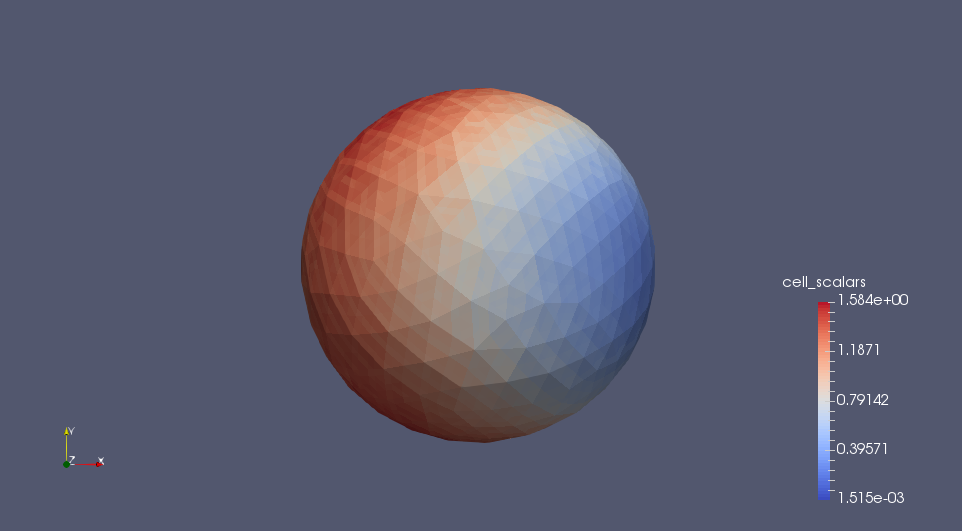
\includegraphics[width=\linewidth]{solution_1.png}
%  \caption{A really Awesome Image}\label{fig:awesome_image1}
\endminipage\hfill
\minipage{0.32\textwidth}
  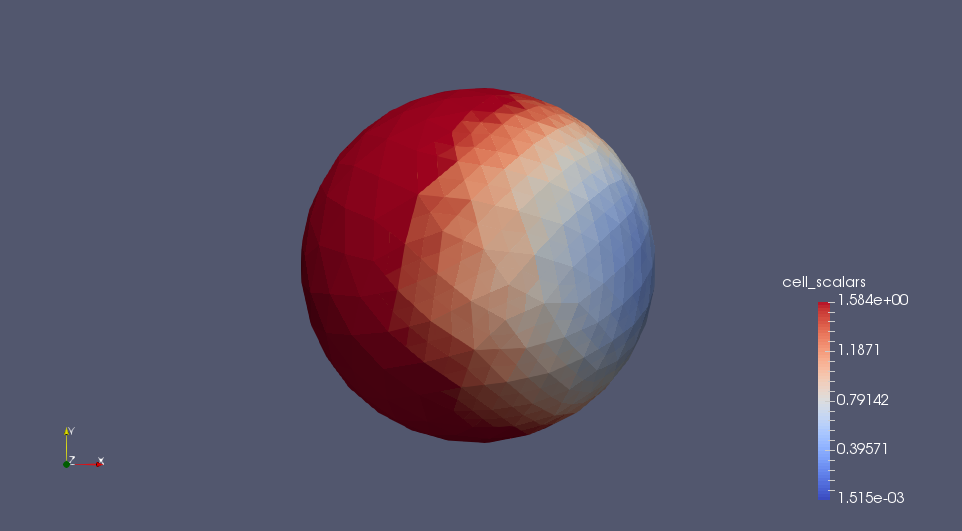
\includegraphics[width=\linewidth]{solution_2.png}
%  \caption{A really Awesome Image}\label{fig:awesome_image2}
\endminipage\hfill
\minipage{0.32\textwidth}
  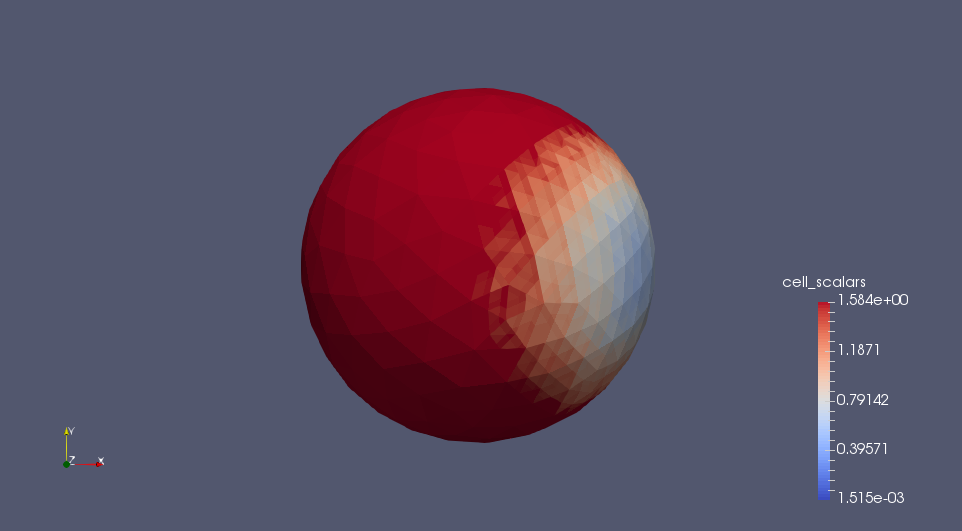
\includegraphics[width=\linewidth]{solution_3.png}
%  \caption{A really Awesome Image}\label{fig:awesome_image2}
\endminipage\hfill
\caption{Numerical solution for hyperbolic problem in 4D. Slices for $t = 0.1$ (left), $t = 0.5$ (middle) and $t = 0.9$ (right).}
\end{figure}

%\newpage

%\section{Acknowledgements}
%
%\section{To-do list:}
%\begin{itemize}
%	\item Rewrite the introduction
%	\item Add references to introduction
%	\item Check the figure references
%	\item Proof read
%\end{itemize}


\begin{thebibliography}{100}

\bibitem{cfosls_code}
CFOSLS, https://github.com/CFOSLS/mfem.

\bibitem{our_cfosls_paper}
K. Voronin, C.-S. Lee, M. Neumueller, P. Sepulveda, P.S. Vassilevski. Space-time discretizations using constrained first-order system least squares (CFOSLS), Journal of Comp. Physics, Volume 373, p. 863-876, https://doi.org/10.1016/j.jcp.2018.07.024

\bibitem{amr_cfosls_report}
K. Voronin. Report on the adaptive mesh refinement strategies for the constrained first-order system least-squares (CFOSLS).

\bibitem{Behr}
M. Behr. Simplex Space-Time Meshes in Finite Element Simulations,
Int. J. Numer. Meth. Fluids 2008; 57:1421–1434.

\bibitem{NeumuellerViz}
M. Neumueller, O. Steinbach. Refinement of flexible space–time finite element meshes and discontinuous Galerkin methods, Comput. Visual Sci. (2011) 14:189–205, DOI 10.1007/s00791-012-0174-z

\bibitem{NeumuellerMeshgen}
E. Karabelas, M. Neumueller. Generating admissible space-time meshes for moving domains in $d + 1$-dimensions, https://arxiv.org/abs/1505.03973.

\bibitem{CFOSLS}
M. Neumueller, P.S. Vassilevski, U. Villa. Space-time CFOSLS Methods with AMGe Upscaling, 23th International Conference on Domain Decomposition Methods, 2016 (not sure?).
CFOSLS references

\bibitem{RT}
P.A. Raviart, J.M. Thomas. A mixed finite element method for second order elliptic problems, Mathematical Aspects of the Finite Element Method, (I. Galligani, E. Magenes, eds.), Lectures Notes in
Math. 606, Springer Verlag, 1977.

\bibitem{hypre}
HYPRE: A library of High Performance Preconditioners. https://www.llnl.gov/CASC/hypre.

\bibitem{mfem}
Modular Finite Element Methods (MFEM), http://mfem.org.

\bibitem{qhull}
Qhull. http://www.qhull.org

\bibitem{paraview}
U. Ayachit. The ParaView Guide: A Parallel Visualization Application. Kitware Inc., Clifton Park (2015).

\bibitem{vtk}
W. Schroeder, K. Martin, B. Lorensen. The Visualization Toolkit (4th ed.), Kitware, (2006), ISBN 978-1-930934-19-1.

\bibitem{coeus}
Coeus cluster. http://www.pi4cs.org/equipment.

\end{thebibliography}

\end{document}